%-------------------------
%device-revisited.tex
%(c) H.Buchmann FHNW 2018
%export TEXINPUTS=${HOME}/fhnw/edu/:${HOME}/fhnw/edu/tinL/config/latex:${HOME}/fhnw/edu/config//:
%-------------------------
\documentclass{beamer}
\usepackage{latex/beamer}
%---------------------
%local defines
%(c) H.Buchmann FHNW 2009
%$Id$
%---------------------
\newcommand{\target} {\beaglebone\xspace}
\newcommand{\targetS}{{\bf BBG}\xspace}
\newcommand{\host}   {{\em Host}\xspace}
\newcommand{\targetroot} {{\bf target-root}\xspace}
\newcommand{\kernel} {{\bf kernel}\xspace}
\renewcommand{\c}{{\bf C}\xspace}
\newcommand{\cpp}{{\bf C++}\xspace}
\newcommand{\posix}{{\bf POSIX}\xspace}

\input{/home/buchmann/latex/dirtree/dirtree.tex}
\usepackage{svg}
\usepackage[absolute]{textpos}
\setlength{\TPHorizModule}{1mm}
\setlength{\TPVertModule}{1mm}

\begin{document}


\title[Devices revisited]{Devices revisited}

\frame{\titlepage}

\begin{frame}{Um was geht es ?}{\c und Scripts}
 \begin{itemize}
  \item Verbindung 
  \begin{itemize}
   \item {\em kernel-space} $\leftrightarrow$ {\em user-space}
  \end{itemize}
  \item call-backs
  \begin{itemize}
   \item verschiedene Formen
  \end{itemize}
  \item Info \url[http]{lxr.free-electrons.com}
  \item Schritt f�r Schritt mit \cod{git}
  \begin{itemize}
   \item \cod{git log}
   \item \cod{git show}
  \end{itemize}
 \end{itemize}
\end{frame}

\begin{frame}{Um was geht es ?}
 \begin{itemize}
  \item Kernel-Modules: {\bf L}oadable {\bf K}ernel {\bf M}odule
  \begin{itemize}
   \item \cod{insmod}
   \item \cod{rmmodule}
  \end{itemize}
  \item device
  \begin{itemize}
   \item {\em major} {\em minor}
   \item \cod{devicefile} $=$ {\em major} {\em minor}
  \end{itemize}
  \item {\em kernel-space} $\leftrightarrow$ {\bf devicefile} $\leftrightarrow$ {\em user-space}
 \end{itemize}
\end{frame}

\begin{frame}{Um was geht es ?}{kernel-space $\leftrightarrow$ user-space}
\begin{block}{Wie merkt der {\em kernel}-space}
\begin{itemize}
 \item ob ein {\bf LKM}
 \begin{itemize}
  \item eingef�gt
  \item entfernt 
 \end{itemize}
 wird
\end{itemize}
\end{block}
\begin{block}{Wie merkt der {\em user}-space}
 \begin{itemize}
  \item ob sich in einem {\bf LKM}
  \begin{itemize}
   \item etwas tut  
  \end{itemize}
  wird
 \end{itemize}
\end{block}
\end{frame}

\begin{frame}{Setup}{Programmentwicklung}
\begin{tabular}{l|l}
\multicolumn{1}{c|}{\host} & \multicolumn{1}{c}{\targetS}\\
\hline
start				& \\
\cod{minicom -D/dev/ttyUSB0} 	&\\
				& start\\
        			& \cod{ifconfig usb0 192.168.7.7}\\
        			& \cod{/sbin/sshd}\\
\cod{ssh root@192.168.7.7}      &\\
\cod{sshfs root@192.168.7.7: mount} &\\
\hline
\multicolumn{2}{c}{ready to develop}	
\end{tabular}
\end{frame}

\begin{frame}{\cod{simple-device-1.c}}
  \begin{itemize}
   \item init/exit
   \item \cod{struct file\_operations fops;}
  \end{itemize}
\end{frame}

\begin{frame}{\cod{simple-device-2.c}}{empty read/write}
 \begin{itemize}
  \item {\em kernel-space}
  \begin{itemize}
  \item \cod{file\_operations}: read/write
  \begin{itemize}
   \item mit \cod{printk} call-back anzeigen
  \end{itemize}
  \end{itemize}
  \item {\em user-space}
  \begin{itemize}
  \item \cod{mknod device c {\em Major} 0} 
  \item read: \cod{cat device}
  \item write: \cod{echo abcd > device}
  \end{itemize}
 \end{itemize}
\end{frame}

\begin{frame}{\cod{simple-device-3.c}}{read/write}
\begin{center}
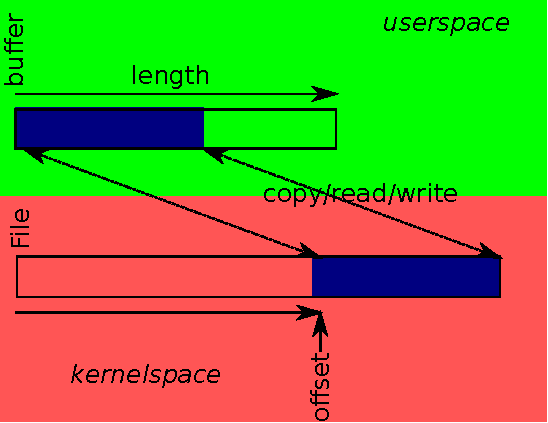
\includegraphics[height=0.375\textheight]{user-kernel-space-copy.pdf}
\end{center}
\begin{itemize}

 \item read/write:
 \begin{itemize}
  \item \cod{copy\_to\_user}/\cod{copy\_from\_user}
  \item das Zusammenspiel:
  \begin{itemize}
   \item \cod{len}m\cod{*ofs}
  \end{itemize}
 \end{itemize}
\end{itemize}
\end{frame}

\begin{frame}{\cod{simple-device-4.c}}{Verbindung mit {\em userspace}: \cod{/sys}}
\begin{itemize}
 \item {\em kernel-space}
 \begin{itemize}
  \item \cod{MODULE\_LICENSE ("{}GPL"{})}
  \item init: \cod{simple\_module=class\_create(THIS\_MODULE,"{}simple\_device"{})}
  \item exit: \cod{class\_destroy(simple\_class)}
 \end{itemize}
 \item {\em user-space}
 \begin{itemize}
  \item \cod{ls /sys/class}
 \end{itemize}
 \item noch keine Informationen in \cod{/sys/class/simple\_device}
\end{itemize}
\end{frame}

\begin{frame}{\cod{simple-device-5.c}}{Verbindung mit {\em userspace}: \cod{/sys}}
 \begin{itemize}
  \item {\em kernel-space}
  \begin{itemize}
   \item init: \cod{device\_create},\cod{KDEV(Major,0)}
   \item exit: \cod{device\_destroy}
  \end{itemize}
  \item {\em user-space}
  \begin{itemize}
   \item \cod{ls /sys/class/simple\_device}
  \end{itemize}
 \end{itemize}
\end{frame}

\begin{frame}{hotplug}
\end{frame}
\end{document}
